


\subsection{Distillation improves performance and enables scaling agents} \label{sec:results_kickstarting}

\begin{figure}[t!]
    \centering
    \begin{subfigure}[b]{0.49\textwidth}
        \centering
        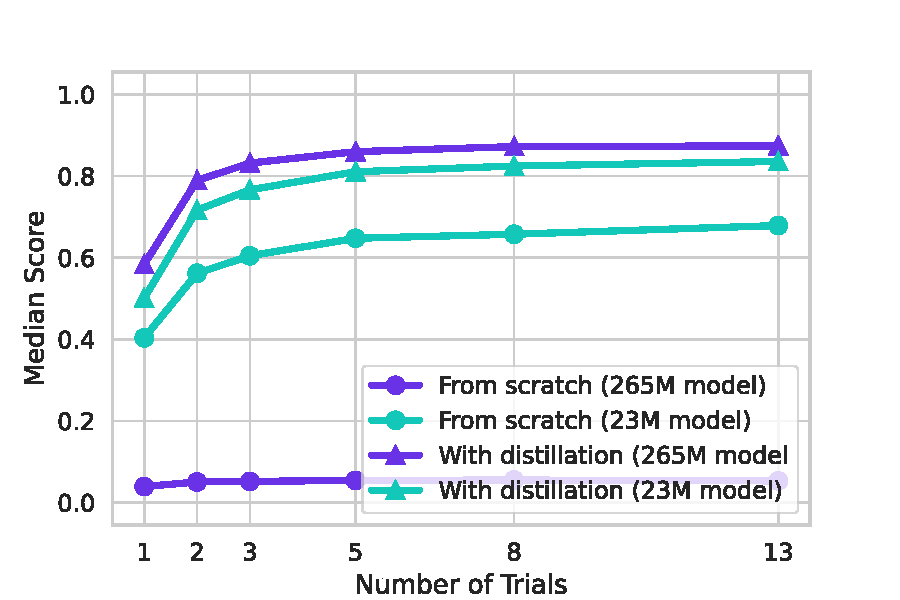
\includegraphics[width=\linewidth]{figures/scaling_from_scratch_vs_distillation_perc50.pdf}
        \vskip -3pt \caption{}
    \end{subfigure}
    \begin{subfigure}[b]{0.49\textwidth}
        \centering
        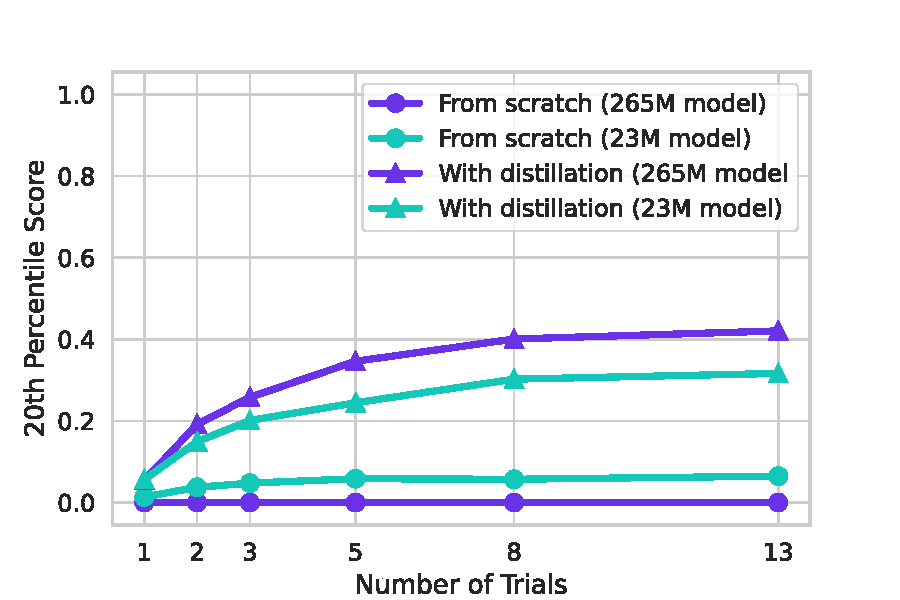
\includegraphics[width=\linewidth]{figures/scaling_from_scratch_vs_distillation_perc20.pdf}
        \vskip -3pt \caption{}
    \end{subfigure}
    \caption{
        Adaptation over increasing numbers of trials when training from scratch or when kickstarting with distillation, for models with 23M and 265M Transformer parameters. Circle markers show training from scratch while triangle markers show training kickstarted with 4 billion frames of distillation. For this ablation, agents were trained in the multi-agent setup described in Section~\ref{sec:results_human_scale_adaptation} and evaluated on the multi-agent test set after 22 billion total training frames.
        \textbf{(a)} Median score.
        \textbf{(b)} 20\textsuperscript{th} percentile score.
    }
\label{fig:scaling_from_scratch_vs_distillation}
\end{figure}

\begin{figure}[t!]
    \centering
    \begin{subfigure}[b]{0.49\textwidth}
        \centering
        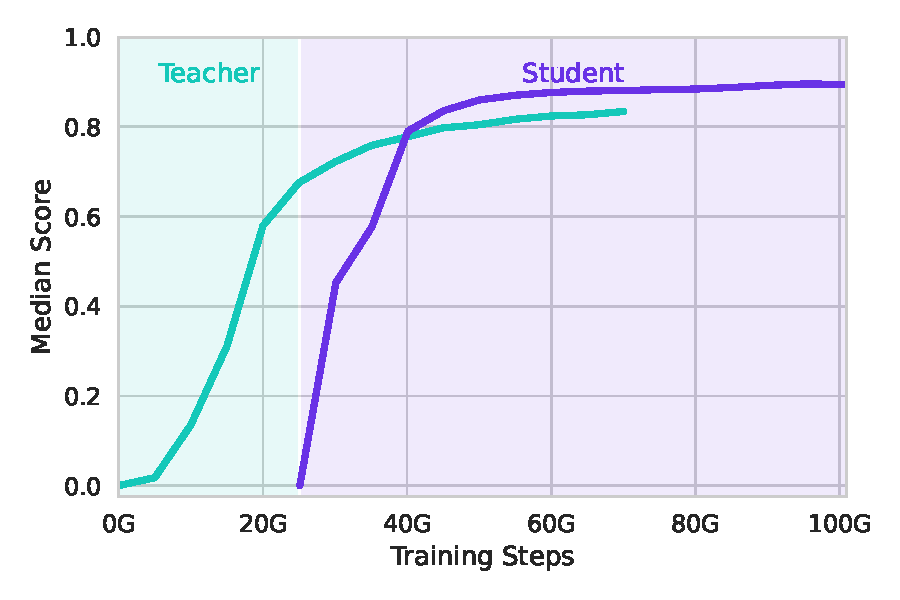
\includegraphics[width=\linewidth]{figures/distillation/distilation_2gen_percentile50_False.pdf} 
        \vskip -3pt \caption{}
    \end{subfigure}
    \begin{subfigure}[b]{0.49\textwidth}
        \centering
        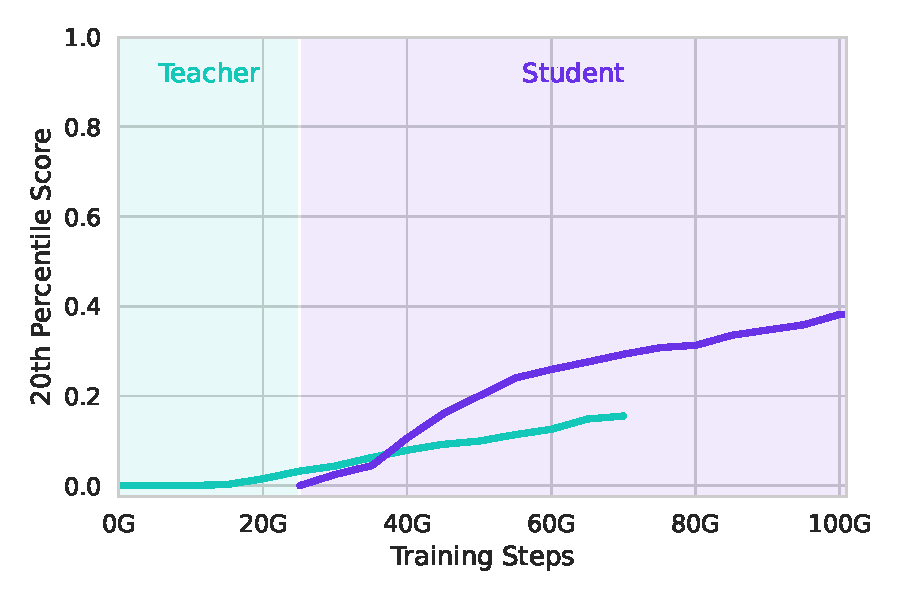
\includegraphics[width=\linewidth]{figures/distillation/distilation_2gen_percentile20_False.pdf} 
        \vskip -3pt \caption{}
    \end{subfigure}
    \caption{
        Normalised last-trial score for $k=13$ using the 23M parameter Transformer-XL. The teacher is trained from scratch, while the otherwise identical student is distilled from a snapshot of the teacher, taken after 25 billion steps of training. The $x$-axis counts the combined amount of experience, including experience used to train the teacher. The comparison shows that distillation can greatly increase the performance of the student, even if the combined amount of experience and updates are equivalent. This is true for median score~\textbf{(a)}, but even more so for the 20\textsuperscript{th} percentile~\textbf{(b)}. 
    }
    \label{fig:distillation}
\end{figure}

All of the scaling comparison experiments shown in the previous section use an identical distillation teacher for the first frames of training, as detailed in Appendix \ref{app:scaling_distillation_teacher}. Now, we look at the role distillation plays in scaling. In short, we find that kickstarting training with a distillation period is crucial when scaling up model size. As shown in Figure~\ref{fig:scaling_from_scratch_vs_distillation}, training a $265$M parameter Transformer model without distillation results in poor performance compared to a much smaller $23$M parameter Transformer trained in the same way. However, when training with distillation from a $23$M parameter teacher for the first 4 billion training frames, the $265$M model clearly outperforms the $23$M variant. See experiment details in Appendix \ref{app:distillation-exp}.

Additionally, we find that even when the model size is the same for both student and teacher, we observe large gains from distillation, for a constant total frame budget (Figure \ref{fig:distillation}). We speculate that this is due to bad representations learned early on by the student agent~\citep{nikishin2022primacy, cetin22stabilizing}, which can be avoided by using distillation. This is also consistent with findings in offline RL, where additional data is often required to effectively scale the model \citep{reid2022wikipedia}. The effect is largest for the first round of distillation, with diminishing returns in subsequent rounds of distillation (Figure \ref{app:repeated_distillation}).